The solution architecture is based on the suggested architecture in Figure 4.1 of the compendium [\cite{compendium}, p. 115].
In order to support a larger instruction set, the solution architecture has been expanded somewhat.
The main differences are that the ALU control unit and the main control unit have been merged, and that a branch controller has been added to take care of branching logic.
The architecture of the presented solution processor is illustrated in figure \ref{figure:cpu-architecture}.

In figure \ref{figure:cpu-architecture}, each box corresponds to an architecture component.
Larger components have their names written the top of each box.
Smaller components have hovering labels showing their names.
The left side of a box is used for input signals, and the right side of the box is used for output signals.
The exception to this rule are the muxes, which use the classic pill-style mux diagrams, with input signals coming in through the top and bottom.


\begin{figure}[h!]
	\begin{center}
		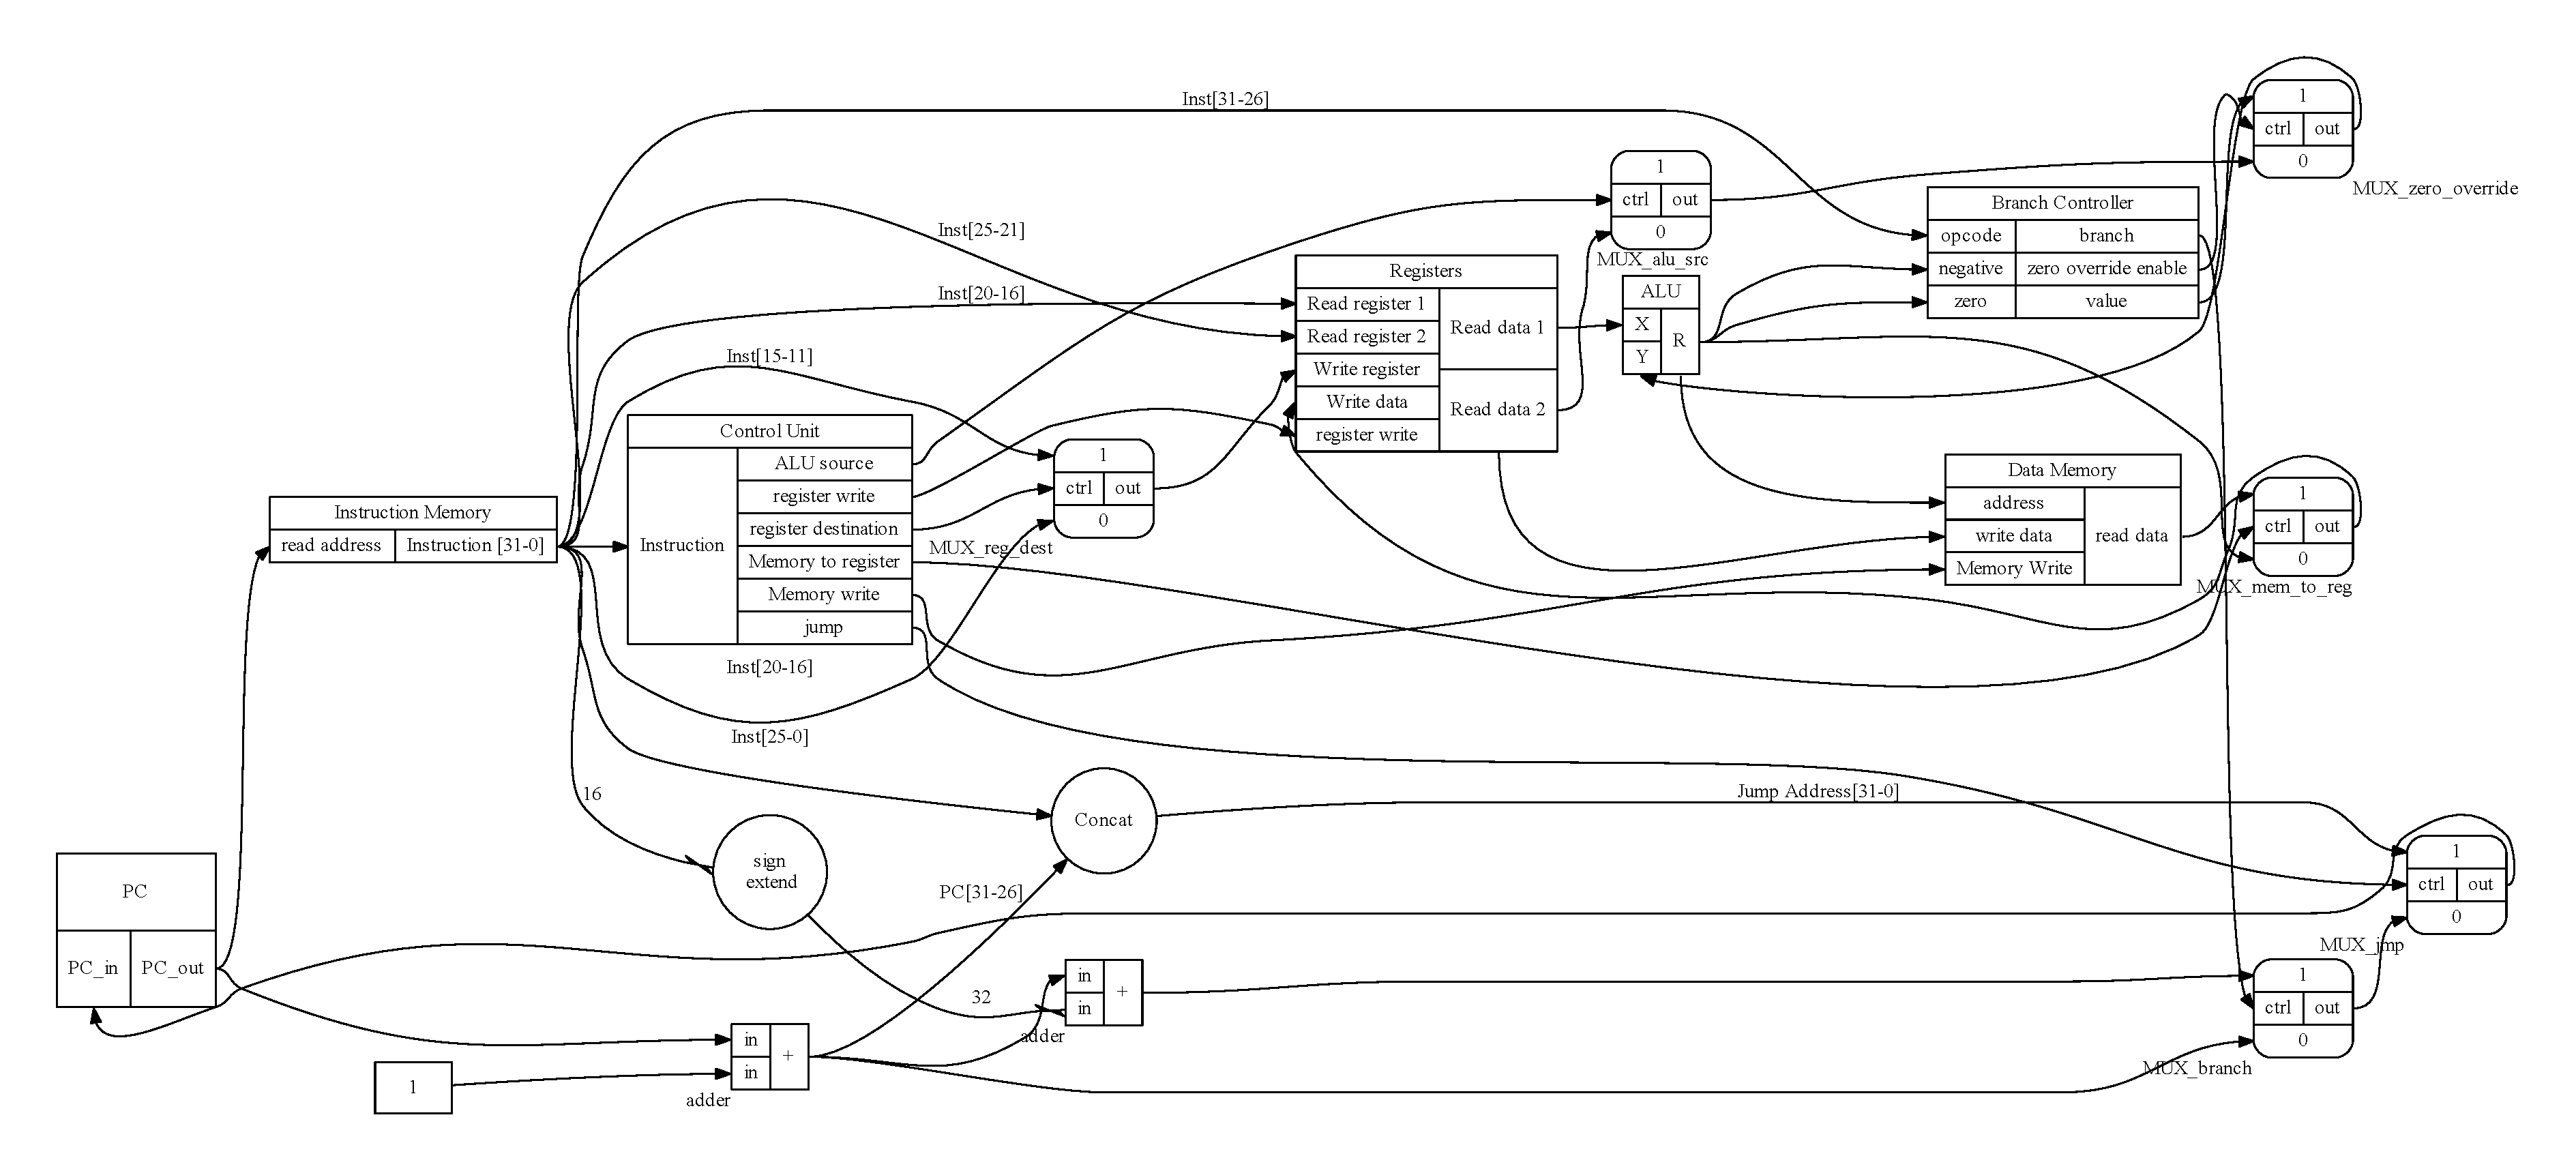
\includegraphics[keepaspectratio, height=\textheight, width=\textwidth]{graphics/cpu-architecture/cpu-architecture.pdf}
		\caption{Architecture of the solution processor.}
		\label{figure:cpu-architecture}
	\end{center}
\end{figure}
